\documentclass[12pt, a4paper]{report}
\usepackage{epsfig}
\usepackage{subfigure}
%\usepackage{amscd}
\usepackage{amssymb}
\usepackage{amsbsy}
\usepackage{amsmath}
\usepackage{amsthm}
\usepackage{framed}
\usepackage{subfiles}
%\usepackage[dvips]{graphicx}
\usepackage{natbib}
\bibliographystyle{chicago}
\usepackage{vmargin}
% left top textwidth textheight headheight
% headsep footheight footskip
\setmargins{3.0cm}{2.5cm}{15.5 cm}{22cm}{0.5cm}{0cm}{1cm}{1cm}
\renewcommand{\baselinestretch}{1.5}
\pagenumbering{arabic}
\theoremstyle{plain}
\newtheorem{theorem}{Theorem}[section]
\newtheorem{corollary}[theorem]{Corollary}
\newtheorem{ill}[theorem]{Example}
\newtheorem{lemma}[theorem]{Lemma}
\newtheorem{proposition}[theorem]{Proposition}
\newtheorem{conjecture}[theorem]{Conjecture}
\newtheorem{axiom}{Axiom}
\theoremstyle{definition}
\newtheorem{definition}{Definition}[section]
\newtheorem{notation}{Notation}
\theoremstyle{remark}
\newtheorem{remark}{Remark}[section]
\newtheorem{example}{Example}[section]
\renewcommand{\thenotation}{}
\renewcommand{\thetable}{\thesection.\arabic{table}}
\renewcommand{\thefigure}{\thesection.\arabic{figure}}
\title{Research notes: linear mixed effects models}
\author{ } \date{ }


\begin{document}
	\author{Kevin O'Brien}
	\title{Method Comparison Studies}
	
	\addcontentsline{toc}{section}{Bibliography}
	
	\tableofcontents
	
	
	
	%\subsection{Bartko's Bradley-Blackwood Test}
	%
	%\begin{itemize}
	%	\item The Bradley Blackwood test is a simultaneous test for bias and
	%	precision. They propose a regression approach which fits D on M,
	%	where D is the difference and average of a pair of results.
	%	\item Both beta values, the intercept and slope, are derived from the respective means and
	%	standard deviations of their respective data sets.
	%	\item We determine if the respective means and variances are equal if
	%	both beta values are simultaneously equal to zero. The Test is
	%	conducted using an F test, calculated from the results of a
	%	regression of D on M.
	%	\item We have identified this approach  to be examined to see if it can
	%	be used as a foundation for a test perform a test on means and
	%	variances individually.
	%	\item Russell et al have suggested this method be used in conjunction
	%	with a paired t-test, with estimates of slope and intercept.
	%\end{itemize}
	%subsection{t-test}
	
\chapter{Formal Models and Tests}


\section{Formal Models and Tests}
The Bland-Altman plot is a simple tool for inspection of data, and
\citet{Kinsella} comments on the lack of formal testing offered by
that approach. It is upon the practitioner opinion to judge the outcome of the approach. An approach proposed by \citet{BA83} is a formal test on the
Pearson correlation coefficient of case-wise differences and means
($\rho_{(a,d)}$). According to the authors, this test is equivalent
to the `Pitman-Morgan Test' a key contribution on the subject \citep{ morgan, pitman}. There has
no been no further mention of this particular test in
\citet{BA86}, although \citet{BA99} refers to Spearman's rank
correlation coefficient. \citet{BA99} commented `we do not see a
place for methods of analysis based on hypothesis testing', while also stating that they consider structural equation models to be inappropriate.

%
%For the Grubbs data, the correlation
%coefficient estimate ($r_{(a,d)}$) is 0.2625, with a 95\% confidence
%interval of (-0.366, 0.726) estimated by Fishers `$r$ to $z$'
%transformation \citep*{cohen2013applied}. The null hypothesis ($\rho_{AD}$ =0)
%fail to be rejected. Consequently the null hypothesis of equal
%variances of each method would also fail to be rejected. 
\subsection*{Kinsella's Model}
\citet{Kinsella} formulates a model for
single measurement observations for a method comparison study as a
linear mixed effects model, i.e. model that additively combine
fixed effects and random effects.
\[
Y_{ij} =\quad \mu + \beta_{j} + u_{i} + \epsilon_{ij} \qquad i = 1,\dots,n
\qquad j=1,2\]

The true value of the measurement is represented by $\mu$ while the fixed effect due to method $j$ is $\beta_{j}$.
For simplicity these terms can be combined into single terms; $\mu_{1} = \mu+ \beta_{1}$ and $\mu_{2} = \mu + \beta_{2}$. The inter-method bias is the difference of the two fixed effect terms, $\beta_{1}-\beta_{2}$. Each of the $i$ individuals are assumed to give rise to random error, represented by $u_{i}$. This random effects terms is assumed to have mean zero and be normally distributed with variance $\sigma^2$. There is assumed to be an attendant error for each measurement on each individual, denoted $\epsilon_{ij}$. This is also assumed to have mean zero. The variance of measurement error for both methods are not assumed to be identical for both methods variance,  hence it is denoted $\sigma^2_{j}$. The set of observations ($x_{i},y_{i}$) by methods $X$ and $Y$ are assumed to follow the bivariate normal distribution with expected values $E(x_{i})= \mu_{i}$ and $E(x_{i})= \mu_{i}$ respectively. The variance covariance of the observations $\Sigma$ is given by

\[
\Sigma = \left[
\begin{array}{cc}
\sigma^{2} + \sigma^{2}_{1} & \sigma^{2} \\
\sigma^{2} & \sigma^{2} + \sigma^{2}_{2} \\
\end{array}
\right]
\]

\citet{Kinsella} demonstrates the estimation of the variance terms and relative precisions relevant to a method comparison study, with attendant confidence intervals for both. The measurement model introduced by \citet{Grubbs48,Grubbs73} provides a formal procedure for estimate the variances $\sigma^2$, $\sigma^2_{1}$ and $\sigma^2_{2}$ devices. \citet{Grubbs48} offers estimates, commonly known as Grubbs estimators, for the various variance components. These estimates are maximum likelihood estimates, a statistical concept that shall be revisited in due course.
\begin{eqnarray*}
	\hat{\sigma^{2}} = \sum{\frac{(x_{i}-\bar{x})(y_{i}-\bar{y})}{n-1}} = Sxy\\
	\hat{\sigma^{2}_{1}} = \sum{\frac{(x_{i}-\bar{x})^{2}}{n-1}} =S^{2}x - Sxy  \\
	\hat{\sigma^{2}_{2}} =
	\sum{\frac{(y_{i}-\bar{y})^{2}}{n-1}} = S^{2}y - Sxy
\end{eqnarray*}

% The standard error of these variance estimates are:
% \begin{eqnarray}
% \mbox{var}(\sigma^{2}_{1}) = \frac{2\sigma^{4}_{1}}{n-1} +
% \frac{\sigma^2_{S}\sigma^2_{1}+\sigma^2_{S}\sigma^2_{2}+\sigma^2_{1}\sigma^2_{2}
% }{n-1}\\
% \mbox{var}(\sigma^{2}_{2}) =\quad \frac{2\sigma^{4}_{2}}{n-1} +
% \frac{\sigma^2_{S}\sigma^2_{1}+\sigma^2_{S}\sigma^2_{2}+\sigma^2_{1}\sigma^2_{2}
% }{n-1}\nonumber
% \end{eqnarray}

\citet{Thompson} presents confidence intervals for the relative
precisions of the measurement methods, $\Delta_{j}=
\sigma^2_{S}/\sigma^2_{j}$ (where $j=1,2$), as well as the
variances $\sigma^{2}_{S}, \sigma^{2}_{1}$ and $\sigma^{2}_{2}$,

\begin{eqnarray}
\Delta_{1} >\quad \frac{C_{xy}-
	t(|A|/n-2))^{\frac{1}{2}}}{C_{x}-C_{xy}+
	t(|A|/n-2))^{\frac{1}{2}}}.
\end{eqnarray}

\citet{Thompson} defines $\Delta_{j}$ to be a measure of the
relative precision of the measurement methods, with $\Delta_{j}=
\sigma^2/\sigma^2_{j}$. Thompson also demonstrates how to make statistical inferences about $\Delta_{j}$.
Based on the following identities,
\begin{eqnarray*}
	C_{x}&=&(n-1)S^2_{x},\nonumber\\
	C_{xy}&=&(n-1)S_{xy},\nonumber\\
	C_{y}&=&(n-1)S^2_{y},\nonumber\\
	|A| &=& C_{x}\times C_{y} - (C_{xy})^2,\nonumber
\end{eqnarray*}
\noindent the confidence interval limits of $\Delta_{1}$ are
\begin{eqnarray}
\Delta_{1} > \frac{C_{xy}-
	t(\frac{|A|}{n-2}))^{\frac{1}{2}}}{C_{x}-C_{xy}+
	t(\frac{|A|}{n-2}))^{\frac{1}{2}}} \\
\Delta_{1} > \frac{C_{xy}+
	t(\frac{|A|}{n-2}))^{\frac{1}{2}}}{C_{x}-C_{xy}-
	t(\frac{|A|}{n-1}))^{\frac{1}{2}}} \nonumber
\end{eqnarray}
The value $t$ is the $100(1-\alpha/2)\%$ upper quantile of
Student's $t$ distribution with $n-2$ degrees of freedom
\citep{Kinsella}. The confidence limits for $\Delta_{2}$ are found by substituting $C_{y}$ for $C_{x}$ in (1.3).
Negative lower limits are replaced by the value $0$.

%For the interval estimates for the variance components,
%\citet{Thompson} presents three relations that hold simultaneously
%with probability $1-2\alpha$ where $2\alpha=0.01$ or $0.05$.

%\begin{eqnarray*}
%|\sigma^2-C_{xy}K| &\leqslant& M(C_{x}C_{y})^{\frac{1}{2}}\\
%|\sigma^2_{1}-(C_{x}-C_{xy})K|&\leqslant M(C_{x}(C_{x}+C_{y}-2C_{xy}))^{\frac{1}{2}}\nonumber\\
%|\sigma^2_{2}-(C_{y}-C_{xy})K|&\leqslant
%M(C_{y}(C_{x}+C_{y}-2C_{xy}))^{\frac{1}{2}}\nonumber
%\end{eqnarray*}

%\citet{Thompson} contains tables for $K$ and $M$.


\subsection{Classical model for Single Measurements}

\citet{BXC2004} presented a simple model to describe a measurement by method $m$, describing the relationship with its real value. The non-replicate case is considered first, as it is the context of the Bland-Altman plots. This model assumes that inter-method bias is the only difference between the two methods.

This model is based on measurements $y_{mi}$ by method $m=1,2$ on item $i = 1,2 \ldots$. We use the term $item$ to denote an individual, subject or sample, to be measured, being randomly sampled from a population

The classical model is based on measurements $y_{mi}$ by method $m=1,2$ on item $i = 1,2 \ldots$
\begin{equation}
y_{mi}  = \alpha_{m} + \mu_{i} + e_{mi}, \qquad  e_{mi} \sim
\mathcal{N}(0,\sigma^{2}_{m}).
\end{equation}
Here $\alpha_m$ is the fixed effect associated with method $m$,
$\mu_i$ is the true value for item $i$ (fixed effect) and $e_{mi}$ is a random effect term for errors.

The random error term for each response is denoted $\varepsilon_{mir}$ having $\mathrm{E}(\varepsilon_{mir})=0$, $\mathrm{Var}(\varepsilon_{mir})=\varphi^2_m$. All the random effects are assumed independent, and that all replicate measurements are assumed to be exchangeable within each method.

The case-wise differences and means are calculated as $d_{i} =
x_{i}-y_{i}$ and $a_{i} = (x_{i}+y_{i})/2$  respectively. Both
$d_{i}$ and $a_{i}$ are assumed to follow a bivariate normal
distribution with $E(d_{i})= \mu_{d} = \mu_{1} - \mu_{2}$ and
$E(a_{i})= \mu_{a} = (\mu_{1} + \mu_{2})/2$. The variance matrix
$\Sigma_{(a,d)}$ is
\begin{eqnarray}
\Sigma_{(a,d)}= \left[\begin{matrix}
\sigma^{2}_{1}+\sigma^{2}_{2}&\frac{1}{2}(\sigma^{2}_{1}-\sigma^{2}_{2})\\
\frac{1}{2}(\sigma^{2}_{1}-\sigma^{2}_{2})&\sigma^{2}+
\frac{1}{4}(\sigma^{2}_{1}+\sigma^{2}_{2})
\end{matrix} \right].
\end{eqnarray}


Likewise the separate $\alpha$ can not be estimated, only their difference can be estimated as $\bar{d}$ (i.e. the inter-method bias). This model implies that the difference between the paired measurements can be expressed as
\[ d_{i} = y_{1i} - y_{2i} \sim \mathcal{N} (\alpha_{1} - \alpha_{2}, \sigma^2_{1} + \sigma^2_{2}). \]
Importantly, this is independent of the item levels $\mu_i$. As the case-wise differences are of interest, the parameters of interest are the fixed effects for methods $\alpha_{m}$.

\subsection{Statement of a Model}
\citet{BXC2010} presents a useful formulation for comparing two methods $X$ and $Y$, in their measurement of item $i$, where the unknown `true value' is $\tau_i$. Other authors, such as \citet{Kinsella}, present similar formulations of the same model, as well as modified models to account for multiple measurements by each methods on each item, known as replicate measurements.

%	\begin{eqnarray} X_i = \tau_i + \delta_i, \phantom{spacin} \delta_i \sim \mathcal{N}(0,\sigma^2_\delta)\\ Y_i = \alpha + \beta \tau_i + \epsilon_i, \phantom{spaci}  \epsilon_i \sim \mathcal{N}(0,\sigma^2_\epsilon)\end{eqnarray}
%	
In some types of analysis, such as the conversion problems described by \citet{lewis}, an estimate for 
the scaling factor $\beta$ may also be sought. For the time being, we will restrict ourselves to problems where $\beta$ is assumed to be 1. 
\begin{eqnarray}
X_i = \tau_i + \delta_i, \phantom{spacin} \delta_i \sim \mathcal{N}(0,\sigma^2_\delta)\\
Y_i = \alpha + \beta \tau_i + \epsilon_i, \phantom{spaci}  \epsilon_i \sim \mathcal{N}(0,\sigma^2_\epsilon)
\end{eqnarray}

In this formulation, $\alpha$ represents the inter-method bias, and can be estimated as $E(X-Y)$. That is to say, a simple estimate of the inter-method bias is given by the differences between pairs of measurements.  

%Table~\ref{FCTdata} is a good example of possible inter-method bias; the `Fotobalk' consistently recording
%smaller velocities than the `Counter' method. A cursory inspection of the table will indicate a systematic tendency for the Counter method to result in higher measurements than the Fotobalk method. % Consequently one would conclude that there is lack of agreement % between the two methods.








\subsection{Pitman-Morgan Testing}
An early contribution to formal testing in method comparison was
made by both \citet{morgan} and \citet{pitman}, in separate
contributions. The basis of this approach is that if the
distribution of the original measurements is bivariate normal.
Morgan and Pitman noted that the correlation coefficient depends
upon the difference $\sigma^{2}_{1}- \sigma^{2}_{2}$, being zero
if and only if $\sigma^{2}_{1}=\sigma^{2}_{2}$.
Therefore a test of the hypothesis $H: \sigma^{2}_{1}=\sigma^{2}_{2}$ is equivalent to a test of the hypothesis $H: \rho(a,d) = 0$. This corresponds to the well-known $t-$test for a correlation coefficient with $n-2$ degrees of freedom. 

The Pitman-Morgan test for equal variances is based on the correlation of $D$ with $S$. The correlation coefficient is zero if, and only if, the variances are equal. The test statistic is the familiar t-test with $n-2$ degree of freedom. 

This test assess the equality
of population variances. Pitman's test tests for zero correlation between the sums and products. The basis of this approach is that the distribution of the original measurements is bivariate normal.
Correlation between differences and means is a test statistics for
the null hypothesis of equal variances given bivariate normality.



The test of the hypothesis that the variances $\sigma^2_1$ and $\sigma^2_2$ are equal, which was devised concurrently by \citet{pitman} and \citet{morgan}, 
is based on the correlation of the casewise-differences and sums, $d$ with $s,$ the coefficient being $ \rho_{(d,s)} = (\sigma^2_1 -\sigma^2_2) / ( \sigma_D \sigma_S ),$ which is zero if, and only
if, $\sigma^2_1 = \sigma^2_2.$ 

The classical Pitman-Morgan test can be adapted as a hypothesis test of equal variance for both methods, based on the correlation value $\rho_{a,d}$;

\begin{equation}
\rho(a,d)=\quad\frac{\sigma^{2}_{1}-\sigma^{2}_{2}}{\sqrt{(\sigma^{2}_{1}+\sigma^{2}_{2})(4\sigma^{2}_{S}+\sigma^{2}_{1}+\sigma^{2}_{2})}}.
\end{equation}

\citet{Bartko} describes the Morgan-Pitman test as identical to the test of the slope equal to zero in the regression of $Y_{i1}$ on $Y_{12}$, a result that can be derived using straightforward algebra. The Pitman-Morgan test is equivalent to the marginal test of the slope estimate in \citet{BB89}.

\citet{Bartko} discusses the use of the well known paired sample $t$ test to test for inter-method bias; $H: \mu_{d}=0$. The test statistic is distributed a $t$ random variable with $n-1$ degrees of freedom. Only if the two methods show comparable precision then the paired sample student t-test is appropriate for testing the inter-method bias.





\section{Bradley Blackwood}

\citet{BB89} offers a formal simultaneous hypothesis test for the
mean and variance of two paired data sets. Using simple linear
regression of the differences of each pair against the sums, a
line is fitted to the model, with estimates for intercept and
slope ($\hat{\beta}_{0}$ and $\hat{\beta}_{1}$). The null
hypothesis of this test is that the mean ($\mu$) and variance
($\sigma^{2}$) of both data sets are equal if the slope and
intercept estimates are equal to zero(i.e $\sigma^{2}_{1} =
\sigma^{2}_{2}$ and $\mu_{1}=\mu_{2}$ if and only if $\beta_{0}=
\beta_{1}=0$ )

A test statistic is then calculated from the regression analysis
of variance values \citep{BB89} and is distributed as `$F$' random
variable. The degrees of freedom are $\nu_{1}=2$ and $\nu_{1}=n-2$
(where $n$ is the number of pairs). The critical value is chosen
for $\alpha\%$ significance with those same degrees of freedom.
\citet{Bartko} amends this approach for use in method
comparison studies, using the averages of the pairs, as opposed to
the sums, and their differences. This approach can facilitate
simultaneous usage of test with the Bland-Altman technique.
Bartko's test statistic take the form:
\[ F.test = \frac{(\Sigma d^{2})-SSReg}{2MSReg}
\]
% latex table generated in R 2.6.0 by xtable 1.5-5 package
% Mon Aug 31 15:53:51 2009
\begin{table}[ht]
	\begin{center}
		\begin{tabular}{lrrrrr}
			\hline
			& Df & Sum Sq & Mean Sq & F value & Pr($>$F) \\
			\hline
			Averages & 1 & 0.04 & 0.04 & 0.74 & 0.4097 \\
			Residuals & 10 & 0.60 & 0.06 &  &  \\
			\hline
		\end{tabular}
		\caption{Regression ANOVA of case-wise differences and averages
			for Grubbs Data}
	\end{center}
\end{table}
%(calculate using R code $qf(0.95,2,10)$).

For the Grubbs data, $\Sigma d^{2}=5.09 $, $SSReg = 0.60$ and
$MSreg=0.06$ Therefore the test statistic is $37.42$, with a
critical value of $4.10$. Hence the means and variance of the
Fotobalk and Counter chronometers are assumed to be simultaneously
equal.

Importantly, this approach determines whether there is both
inter-method bias and precision present, or alternatively if there
is neither present. It has previously been demonstrated that there
is a inter-method bias present, but as this procedure does not
allow for separate testing, no conclusion can be drawn on the
comparative precision of both methods.



%This application of the
%Grubbs method presumes the existence of this condition, and necessitates
%replication of observations by means external to and independent of the first
%means. The Grubbs estimators method is based on the laws of propagation of
%error. By making three independent simultaneous measurements on the same
%physical material, it is possible by appropriate mathematical manipulation of
%the sums and differences of the associated variances to obtain a valid
%estimate of the precision of the primary means. Application of the Grubbs
%estimators procedure to estimation of the precision of an apparatus uses
%the results of a physical test conducted in such a way as to obtain a series
%of sets of three independent observations.


 



%	The case-wise differences are expressed as $d_{i} = y_{1i} - y_{2i}$. Even though the separate variances can not be identified, their sum can be estimated by the empirical variance of the differences, using standard statistical theory. The covariance matrix for case-wise differences can be specified as
%	\[
%	\Sigma = \left( \begin{array}{cc}
%	\sigma^2_1 + \sigma^2_2 &  \frac{1}{2}(\sigma^2_1 - \sigma^2_2) \\
%	\frac{1}{2}(\sigma^2_1 - \sigma^2_2) &   \sigma^2_b + \frac{1}{4}(\sigma^2_1 + \sigma^2_2)
%	\end{array}\right).
%	\]

% \[ y_{mi} =  \alpha_{m}  + \mu_{i} + e_{mi}  \]
% Importantly these variance covariance structures are central to ARoy2009 methodology.
% \citet{ARoy2009} proposes a series of hypothesis tests based on these matrices as part of her methodology. These tests shall be reverted to in due course.

%	The standard deviation of the differences of variables $a$ and $b$ is computed as
%	\[
%	\mbox{var}(a - b) = \mbox{var} ( a )  + \mbox{var} ( b ) - 2\mbox{cov} ( a ,b )
%	\]





\subsection{Blackwood-Bradley Model} 
\citet{BB89} construct the conditional expectation of D given S as linear model. They used this result to propose a test of the joint hypothesis of the mean difference and equal variances. If the intercept and slope estimates are zero, the two methods have the same mean and variance.

Using simple linear regression of the differences of each pair against the sums, a	line is fitted to the model, with estimates for intercept and slope ($\hat{\beta}_{0}$ and $\hat{\beta}_{1}$). The null	hypothesis of this test is that the mean ($\mu$) and variance ($\sigma^{2}$) of both data sets are equal if the slope and intercept estimates are equal to zero(i.e $\sigma^{2}_{1} =
\sigma^{2}_{2}$ and $\mu_{1}=\mu_{2}$ if and only if $\beta_{0}=
\beta_{1}=0$ )	


\citet{BB89} have developed a regression based procedure for
assessing the agreement. This approach performs a simultaneous test for the equivalence of
means and variances of the respective methods. The Bradley Blackwood test is a simultaneous test for bias and
precision. They propose a regression approach which fits $D$ on $M$, where $D$ is the difference and average of a pair of results. 
\begin{eqnarray}
D = (X_{1}-X_{2}) \\
M = (X_{1} + X_{2}) /2
\end{eqnarray}

Using simple linear regression of the differences of each pair against the sums, a line is fitted to the model, with estimates for intercept and slope ($\hat{\beta}_{0}$ and $\hat{\beta}_{1}$).
%We have identified
%this approach  to be examined to see if it can be used as a %foundation for a test perform a test on
%means and variances individually.

The Bradley Blackwood Procedure fits D on M as follows:\\
\begin{equation}
D = \beta_{0} + \beta_{1}M
\end{equation}
This technique offers a formal simultaneous hypothesis test for the mean and variance of two paired data sets. The null hypothesis of this test is that the mean ($\mu$) and variance ($\sigma^{2}$) of both data sets are equal if the slope and intercept estimates are equal to zero(i.e $\sigma^{2}_{1} =
\sigma^{2}_{2}$ and $\mu_{1}=\mu_{2}$ if and only if $\beta_{0}=
\beta_{1}=0$).

Both regression coefficients are derived from the respective means and
standard deviations of their respective data sets. We determine if the respective means and variances are equal if both beta values are simultaneously equal to zero. The test is conducted using an F test, calculated from the results of a regression of D on M.

%	\textbf{Russell et al} have suggested this method be used in conjunction with a paired t-test, with estimates of slope and intercept.


\subsection{Model for Replicate Measurements}



We generalize the single measurement model for the replicate measurement case, by additionally specifying replicate values. Let $y_{mir}$ be the $r-$th replicate measurement for item $i$ made by method $m$. Further to \citet{barnhart} fixed effect can be expressed with a single term $\alpha_{mi}$, which incorporate the true value $\mu_i$.

\[ y_{mir} = \mu_{i} + \alpha_{m} + e_{mir}  \]

Combining fixed effects \citep{barnhart}, we write,

\[ y_{mir} = \alpha_{mi} + e_{mir}.\]

The following assumptions are required
$e_{mir}$ is independent of the fixed effects with mean $\mbox{E}(e_{mir}) = 0$.
Further to \citet{barnhart} between-item and within-item variances $\mbox{Var}(\alpha_{mi}) = \sigma^2_{Bm}$ and $\mbox{Var}(e_{mir}) = \sigma^2_{Wm}$		

\subsection{Statistical Model For Replicate Measurements}
Let $y_{Aij}$ and $y_{Bij}$ be the $j$th repeated observations of the variables of interest $A$ and $B$ taken on the $i$th item. The number of repeated measurements for each variable may differ for each individual.
Both variables are measured on each time points. Let $n_{i}$ be the number of observations for each variable, hence $2\times n_{i}$ observations in total.

It is assumed that the pair $y_{Aij}$ and $y_{Bij}$ follow a bivariate normal distribution.
\begin{eqnarray}
\left(
\begin{array}{c}
y_{Aij} \\
y_{Bij} \\
\end{array}
\right) \sim \mathcal{N}(
{\mu}, {\Sigma})\mbox{   where } {\mu} = \left(
\begin{array}{c}
\mu_{A} \\
\mu_{B} \\
\end{array}
\right)
\end{eqnarray}
The matrix ${\Sigma}$ represents the variance component matrix between response variables at a given time point $j$.
\begin{equation}
{\Sigma} = \left( \begin{array}{cc}
\sigma^2_{A} & \sigma_{AB} \\
\sigma_{AB} & \sigma^2_{B}\\
\end{array}\right)
\end{equation}
$\sigma^2_{A}$ is the variance of variable $A$, $\sigma^2_{B}$ is the variance of variable $B$ and $\sigma_{AB}$ is the covariance of the two variable. It is assumed that ${\Sigma}$ does not depend on a particular time point, and is the same over all time points.



\subsection{Carstensen's Model for Replicate Measurements}



%If the exact cause of disagreement between the two methods is not of interest, then the overall vaiability test $H_4$ %is an alternative to testing $H_2$ and $H_3$ separately.


\citet{BXC2008} develop their model from a standard two-way analysis of variance model, reformulated for the case of replicate measurements, with random effects terms specified as appropriate. 
For the replicate case, an interaction term $c$ is added to the model, with an associated variance component. Their model describing $y_{mir} $, again the $r$th replicate measurement on the $i$th item by the $m$th method ($m=1,2,$ $i=1,\ldots,N,$ and $r = 1,\ldots,n$), can be written as
\begin{equation}\label{BXC-model}
y_{mir}  = \alpha_{m} + \mu_{i} + a_{ir} + c_{mi} + \epsilon_{mir}.
\end{equation}

The fixed effects $\alpha_{m}$ and $\mu_{i}$ represent the intercept for method $m$ and the `true value' for item $i$ respectively. The random-effect terms comprise an item-by-replicate interaction term $a_{ir} \sim \mathcal{N}(0,\varsigma^{2})$, a method-by-item interaction term $c_{mi} \sim \mathcal{N}(0,\tau^{2}_{m}),$ and model error terms $\varepsilon_{mir} \sim \mathcal{N}(0,\varphi^{2}_{m}).$ All random-effect terms are assumed to be independent. For the case when replicate measurements are assumed to be exchangeable for item $i$, $a_{ir}$ can be removed. 


The model expressed in (2) describes measurements by $m$ methods, where $m = \{1,2,3\ldots\}$. Based on the model expressed in (2), \citet{BXC2008} compute the limits of agreement as
\[
\alpha_1 - \alpha_2 \pm 2 \sqrt{ \tau^2_1 +  \tau^2_2 +  \varphi^2_1 +  \varphi^2_2 }
\]

\citet{BXC2008} notes that, for $m=2$, separate estimates of $\tau^2_m$ can not be obtained. To overcome this, the assumption of equality, i.e. $\tau^2_1 = \tau^2_2$ is required.
\begin{equation}
y_{mir}  = \alpha_{m} + \mu_{i} + c_{mi} + e_{mir}, \qquad  e_{mi}
\sim \mathcal{N}(0,\sigma^{2}_{m}), \quad c_{mi} \sim \mathcal{N}(0,\tau^{2}_{m}).
\end{equation}

%Of particular importance is terms of the model, a true value for item $i$ ($\mu_{i}$). The fixed effect of Roy's model comprise of an intercept term and fixed effect terms for both methods, with no reference to the true value of any individual item. 
%A distinction can be made between the two models: Roy's model is a standard LME model, whereas Carstensen's model is a more complex additive model.



\section{Regression Methods}
Conventional regression models are estimated using the ordinary
least squares (OLS) technique, and are referred to as `Model I
regression' \citep{CornCoch,ludbrook97}. A key feature of Model I
models is that the independent variable is assumed to be measured
without error. As often pointed out in several papers
\citep{BA83,ludbrook97}, this assumption invalidates simple linear
regression for use in method comparison studies, as both methods
must be assumed to be measured with error.

Errors-in-variables models or measurement errors models are regression models that account for measurement errors in the independent variables, as well as the dependent variable.


The use of regression models that assumes the presence of error in
both variables $X$ and $Y$ have been proposed for use instead
\citep{CornCoch,ludbrook97}. These methodologies are collectively
known as `Model II regression'. They differ in the method used to
estimate the parameters of the regression.

Regression estimates depend on formulation of the model. A
formulation with one method considered as the $X$ variable will
yield different estimates for a formulation where it is the $Y$
variable. With Model I regression, the models fitted in both cases
will entirely different and inconsistent. However with Model II
regression, they will be consistent and complementary.





	


\section{Error In Variable Models}
\citet{CornCoch} argue for the use of methods that based on
the assumption that both methods are imprecisely measured ,and
that yield a fitting that is consistent with both '$X$ on $Y$' and
'$Y$ on $X$' formulations. These methods uses alternatives to the
OLS approach to determine the slope and intercept.
	
\citet{CornCoch} comparing the three methods, citing studies by other authors, concluding that Deming regression is the most useful of these methods. They found the Bartlett method to be flawed in determining slopes.
	
Model II regression is suitable for method comparison studies, but it is more difficult to execute. Both Model I and II regression models are unduly influenced by outliers.

The Bland-Altman plot is uninformative about the comparative influence of proportional bias and fixed bias. Model II approaches, such as Deming regression, can provide independent tests for both types of bias.
		
However the author point out that \emph{ clinical laboratory measurements usually increase in absolute imprecision when larger values are measured.} However one of the assumptions that underline Deming and Mandel regression is constancy of the measurement errors throughout the range of values.
	
	
\section{Deming Regression}
The fundamental flaw of simple linear regression is that it allows for measurement error in one variable only. This causes a downward biased slope estimate. The most commonly known Model II methodology is known as Deming's Regression, an approach that assumes error in both variables, and is recommended by \citet*{CornCoch} as the preferred Model II regression for use in method comparison studies. 
		
Informative analysis for the purposes of method comparison, Deming Regression is a regression technique taking into account uncertainty in both the independent and dependent variables.
	
Deming regression method also calculates a line of best fit for two sets of data. It differs from simple linear regression in that it is derived in a way that factors in for error in the x-axis, as well as the y-axis. The sum of the square of the residuals of both variables are simultaneously minimized. This derivation results in the best fit to minimize the sum of the squares of the perpendicular distances from the data points. Normally distributed error of both variables is assumed, as well as a constant level of imprecision throughout the range of measurements.

The sum of squared distances from measured sets of values to the regression line is minimized at an angle specified by the ratio $\lambda$ of the residual variance of both variables. When $\lambda$ is one, the angle is 45 degrees. In ordinary linear regression, the distances are minimized in the vertical directions \citep{linnet99}.

In cases involving only single measurements by each method, $\lambda$ may be unknown and is therefore assumes a value of one. While this will produce biased estimates, they are less biased than ordinary linear regression.
	
%The Deming regression line is estimated by minimizing the sums of squared deviations in both the x and y directions at an angle determined by the ratio of the analytical standard deviations for both methods.
	
\subsection{Kummel's Estimates}

The appropriate estimates were derived by \citet{Kummel}, but were popularized in the context of medical statistics and clinical chemistry by Deming (1943).
For a given $\lambda$, \citet{Kummel} derived the following estimate that would later be used for the Deming regression slope
parameter. 
\begin{equation}
\hat{\beta} =\quad \frac{S_{yy} - \lambda S_{xx}+[(S_{yy} -
	\lambda S_{xx})^{2}+ 4\lambda S^{2}_{xy}]^{1/2}}{2S_{xy}},
\end{equation}
with $\lambda$ as the variance ratio. The intercept estimate $\alpha$ is simply estimated in the same way as in conventional linear
regression, by using the identity $\bar{Y}-\hat{\beta}\bar{X}$. As stated previously $\lambda$ is often unknown, and therefore must be assumed to equal one. 

\citet{CarollRupert} states that Deming
regression is acceptable only when the precision ratio ($\lambda$, in their paper as $\eta$) is correctly specified, but in practice this is often not the case, with the $\lambda$ being underestimated. Several candidate models, with varying variance ratios may be fitted, and estimates of the slope and intercept are produced. However no model selection information is available to determine the best fitting model.

The measurement error is specified with measurement error variance related as 
$\displaystyle{\lambda =\sigma^2_y/\sigma^2_x}$, where $\sigma^2_x$ and $\sigma^2_y$ is the measurement error variance of the $x$ and $y$ variables, respectively.
The variance of the ratio, $\lambda$, specifies the angle. When $\lambda$ is one, the angle is 45 degrees. 
%In ordinary linear regression, the distances are minimized in the vertical directions \citep{linnet99}. 
This approach would be appropriate when errors in $y$ and $x$ are both caused by measurements, and the accuracy of measuring devices or procedures are known. In cases involving only single measurements by each method, $\lambda$ may be unknown and is therefore assumes a value of one. While this will bias the estimates, it is less biased than ordinary linear regression. Deming regression assumes that the variance ratio $\lambda$ is known. When $\lambda$ is defined as one, (i.e. equal error variances), the approach is equivalent to orthogonal regression.


\subsection{Confidence Intervals}
A $95\%$ confidence interval for the intercept estimate can be
used to test the intercept, and hence fixed bias, is equal to
zero. This hypothesis is accepted if the confidence interval for
the estimate contains the value $0$ in its range. Should this be,
it can be concluded that fixed bias is not present. Conversely, if
the hypothesis is rejected, then it is concluded that the
intercept is non zero, and that fixed bias is present.

Testing for proportional bias is a very similar procedure. The
$95\%$ confidence interval for the slope estimate can be used to
test the hypothesis that the slope is equal to $1$. This hypothesis is accepted if the confidence interval for the estimate contains the value $1$ in its range. If the hypothesis is rejected, then it is concluded that the slope is significant different from $1$ and that a proportional bias exists.

	\subsubsection{Inferences for Deming Regression}

As with conventional regression methodologies, Deming regression calculates an estimate for both the slope and intercept for the fitted line, and standard errors thereof. Therefore there is sufficient information to carry out hypothesis tests on both estimates, that are informative about presence of constant and proportional bias. The test for the intercept estimate acts as a test for the presence of constant bias between both measurement methods. Similarly the test for the slope estimate can be used to formally test proportional bias between the two methods.

The intercept and slope are calculated according to \citet{CornCoch}. The standard errors and confidence intervals are estimated using the jackknife method (Armitage et al., 2002). Bootstrap techniques can be used to obtain confidence intervals for Deming regression estimates. Authors such as 
\citet{carpenter2000bootstrap} and \citet{johnson2001bootstrap} provide relevant insights.

Model selection and diagnostic technique are well developed for classical linear regression methods. Typically an implementation of a linear model fit will be accompanied by additional information, such as the coefficient of determination and likelihood and information criterions, and a regression ANOVA table. Such additional information has not, as yet, been implemented for Deming regression.

%===================================================%



\subsection{Zhang Data}
For convenience, a new data set shall be introduced to demonstrate
Deming regression. Measurements of transmitral volumetric flow
(MF) by doppler echocardiography, and left ventricular stroke
volume (SV) by cross sectional echocardiography in 21 patients
with aortic valve disease are tabulated in \citet{zhang}. This
data set features in the discussion of method comparison studies
in \citet[p.398]{AltmanBook} .


% latex table generated in R 2.6.0 by xtable 1.5-5 package
% Tue Sep 01 13:31:17 2009
\begin{table}[h!]
	\begin{center}
		\begin{tabular}{|c|c|c||c|c|c||c|c|c|}
			\hline
			Patient & MF  & SV  & Patient & MF  & SV  & Patient & MF  & SV \\
			&($cm^{3}$)&  ($cm^{3}$) & &($cm^{3}$)&  ($cm^{3}$) & &($cm^{3}$)&  ($cm^{3}$)
			\\
			\hline
			1 & 47 & 43 &  8 & 75 & 72 &  15 & 90 & 82 \\
			2 & 66 & 70 & 9 & 79 & 92 &  16 & 100 & 100 \\
			3 & 68 & 72 & 10 & 81 & 76 & 17 & 104 & 94 \\
			4 & 69 & 81 & 11 & 85 & 85 &  18 & 105 & 98 \\
			5 & 70 & 60 & 12 & 87 & 82 & 19 & 112 & 108 \\
			6 & 70 & 67 & 13 & 87 & 90 & 20 & 120 & 131 \\
			7 & 73 & 72 & 14 & 87 & 96 &  21 & 132 & 131 \\
			
			\hline
		\end{tabular}
		\caption{Transmitral volumetric flow(MF) and left ventricular
			stroke volume (SV) in 21 patients. (Zhang et al 1986)}
	\end{center}
\end{table}

\begin{figure}[h!]
	% Requires \usepackage{graphicx}
	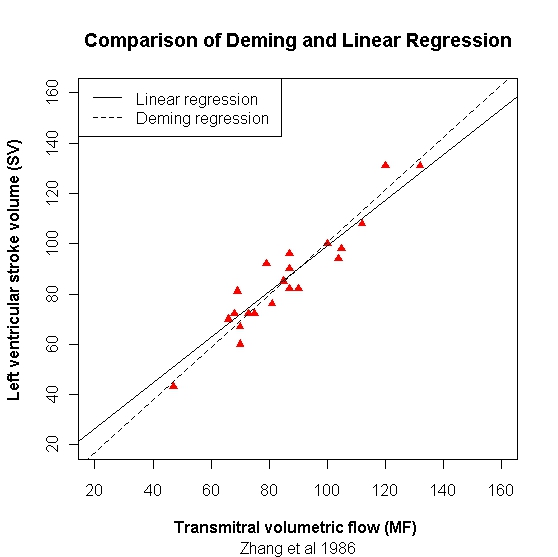
\includegraphics[width=130mm]{images/ZhangDeming.jpeg}
	\caption{Deming Regression For Zhang's Data}\label{ZhangDeming}
\end{figure}




% latex table generated in R 2.6.0 by xtable 1.5-5 package


%\begin{figure}[h!]
%	% Requires \usepackage{graphicx}
%	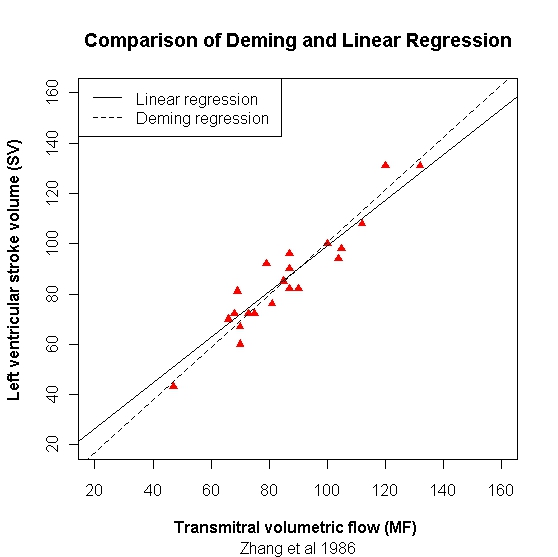
\includegraphics[width=130mm]{images/ZhangDeming.jpeg}
%	\caption{Deming Regression For Zhang's Data}\label{ZhangDeming}
%\end{figure}

	
This ratio can be estimated if multiple measurements were taken with each method, but if only one measurement was taken with each method, it can be assumed to be equal to one.
	

	%\subsection{performance in the presence of oultiers}
	%All least square estimation methods are sensitive to outliers.
	

	
Deming regression is undermined by several factors. Firstly it is computationally complex, and it requires specific software packages to perform calculations. Secondly, in common with all regression methods, Deming regression is vulnerable to outliers. Lastly, Deming regression is uninformative about the comparative precision of two methods of measurement. Most importantly \citet{CarollRupert} states that Deming's regression is acceptable only when the precision ratio ($\lambda$, in their paper as $\eta$) is correctly specified, but in practice this is often not the case, with the $\lambda$ being underestimated. This underestimation leads to an overcorrection for attenuation.

Several candidate models, with varying variance ratios may be fitted, and estimates of the slope and intercept are produced. However no model selection information is available to determine the best fitting model.
	
\subsection{Structural Equation Modelling}
	
Structural equation modelling is a statistical technique used for testing and estimating causal relationships using a combination of statistical data and qualitative causal assumptions. \citet{carrasco2004} describes the structural equation model is a regression approach that allows to estimate a linear 
	regression when independent variables are measured with error.
	The structural equations approach avoids the biased estimation of the slope and intercept that occurs in ordinary least square regression.
	
Several authors, such as \citet{lewis1991}, \citet{gkelly1985}, \citet{voelkel2005} and \citet{hopkins2004bias} advocate the use of SEM methods for method comparison. In \citet{hopkins2004bias}, a critique of the Bland-Altman plot he makes the following remark:


	
	\emph{What's needed for a comparison of two or more measures is a
		generic approach more powerful even than regression to model the
		relationship and error structure of each measure with a latent
		variable representing the true value.}
	
	Hopkins also adds that he himself is collaborating in research utilising SEM and mixed effects modelling. \citet{gkelly1985} advised that \textit{the Structural equations model is used to estimate the linear relationship between new and standards method.
		The Delta method is used to find the variance of the estimated parameters} \citep{gkelly1985}.
	
	
Conversely \citet{BA99} also states that consider structural equation models to be inappropriate. However \citet{BA87} contends that it is unnecessary to perform elaborate statistical analysis, while also criticizing the SEM approach on the basis that it offers insights  on inter-method bias only, and not the variability about the line of equality. 
	\begin{quote}
		\textit{However, it is quite wrong to argue solely from a lack of bias that two methods can be regarded as comparable...
			Knowing the data are consistent with a structural equation with a slope of 1 says something 
			about the absence of bias but nothing about the variability about Y = X (the difference between the measurements), which, as has already been stated, is all that really matters.}
	\end{quote}

\citet{DunnSEME} highlights an important issue regarding using
models such as structural equatio modelling; the identifiability problem. This comes as a result of there being too many parameters to be estimated.
Therefore assumptions about some parameters, or estimators used,
must be made so that others can be estimated. For example, the ratio of the precision of both methods $\lambda=\frac{\sigma^{2}_{1}}{\sigma^{2}_{2}}$
must often be assumed to be equal to $1$ \citep{linnet98}. \citet{DunnSEME} considers methodologies based on two methods with single measurements on each subject as inadequate for a serious
study on the measurement characteristics of the methods, simply because there would not be enough data to allow for a meaningful
analysis. There is, however, a contrary argument that in many
practical settings it is very difficult to get replicate
observations when the measurement method requires an invasive medical
procedure.

%This application of the
%Grubbs method presumes the existence of this condition, and necessitates
%replication of observations by means external to and independent of the first
%means. The Grubbs estimators method is based on the laws of propagation of
%error. By making three independent simultaneous measurements on the same
%physical material, it is possible by appropriate mathematical manipulation of
%the sums and differences of the associated variances to obtain a valid
%estimate of the precision of the primary means. Application of the Grubbs
%estimators procedure to estimation of the precision of an apparatus uses
%the results of a physical test conducted in such a way as to obtain a series
%of sets of three independent observations.



	



\subsubsection{Contention}
Several papers have commented that this approach is underminedwhen the basic assumptions underlying linear regression are not met, the regression equation, and consequently the estimations of bias are undermined. Outliers are a source of error in regression estimates.
	
In method comparison studies, the X variable is a precisely measured reference method. In the \citet{CornCoch} paper. It is argued that criterion may be regarded as the correct value. Other papers dispute this.
	
	

\subsubsection{Expanding the use of Deming Regression for MCS}
As noted before, Deming regression is an important and informative methodology in method comparison studies. For single measurement method comparisons, Deming regression offers a useful complement to LME models.
	

\bibliographystyle{chicago}
\bibliography{2017bib}
\end{document}
